\chapter{Software-Architektur}

Um eine möglichst einfache Wartbarkeit zu garantieren, empfiehlt es sich, die Software logisch aufzubauen. In diesem Kapitel soll nun die Struktur der Anwendung eCourse beschrieben werden. Dabei soll es nicht um die Art und Weise wie der Code geschrieben wurde gehen. Das lässt sich alles in den Codierungsrichtlinen nachlesen.

\section{ERM-Diagramm}
ERM steht für Entity-Relationship-Modell. Dieses Diagramm wird vor der Implementierung der Datenbank erstellt. Dabei wird ein Entwurf der Datenbank gezeichnet. Außerdem dient es dazu im Rahmen der Datenmodellierung relevante Ausschnitte darzustellen. Das ERM für die Anwendung eCourse ist in Abbildung \ref{fib:erm} graphisch aufbereitet.

\begin{figure}[H]
\centering
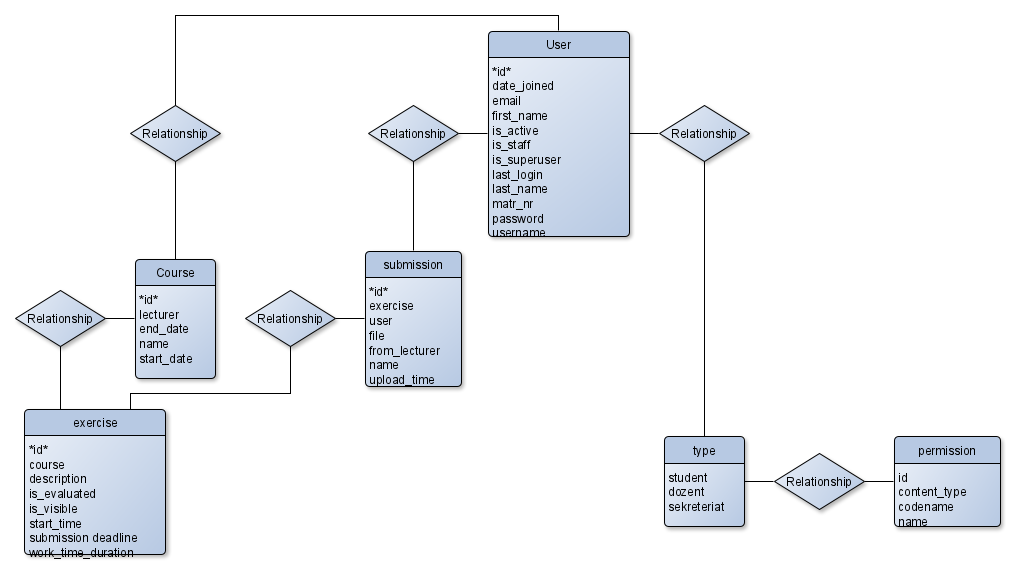
\includegraphics[width=0.9\textwidth]{erm.png}
\caption{ERM im Projekt eCourse}
\label{fib:erm}
\end{figure}

\section{UML-Diagramm}
UML steht für Unified Modeling Language. Ein UML-Diagramm stellt ein Strukturdiagramm dar, auch bekannt unter dem Namen Klassendiagramm. Es wird zur graphischen Modellierung von Klassen, Schnittstellen und deren Beziehungen verwendet. \newline
Das UML für die Anwendung eCourse findet sich aus Übersichtlichkeitsgründen als separate Datei im Dokumentationsordner.